\chapter{Recommendation}\label{ch:recomendations}
This chapter provides various recommendations pertinent to the integration of the \Lone adaptive control algorithm.  These recommendations may be more qualitative than quantitative, but provide experience based guidance for the engineer to better understand the nuances of the \Lone adaptive control algorithm.  Prior to this research, there was very little experientially based guidance on implementation of this algorithm which proved to be the largest barrier for implementing this modern controller.

\section{\Lone Adaptive Control Algorithm Tuning}\label{sec:tuning}
The primary goal of this research was to reduce the complexity of tuning expertise required to get an unknown airframe airborne successfully.  The amount of time required to get the adequate airframe performance using the \Lone algorithm is significantly reduced.  Three primary features need tuning: the adaptation gain, the controller filter, and the companion model.

\subsection{Tuning the Adaptation gain}
Tuning the adaptation gain is fairly intuitive.  The adaptation gain is a function of the loop frequency at which the filter is run so it may only need to be tuned for a given autopilot at a given loop rate and not for every specific aircraft.  Anecdotally, the adaptation gain of 10,000 was used on the Pixhawk1 autopilot running the scheduled loop rate at 100Hz across multiple aircraft without needing to modify.  The primary feedback to the user for tuning this gain resides in the desired movement of the estimated states.  The adaptation gain was set low (1-10) while watching the parameters $(\theta, \omega, \sigma)$ adapt.  The adaptation gain is slowly increased until the desired rate of adaptation as seen in the real time monitoring of the parameters is adequate.  Another approach for tuning the adaptation rate is to increase the gain until parameters start to oscillate between the bounds and then reduce it.  This bang-bang response in the parameter adaptation will show up in the performance of the controller as increased peaks away from zero error between desired and achieved.  In the case of this research, this noise can be hard to identify in the rate control itself and therefore is why monitoring the attitude error helps find the appropriate adaptation gain which is extremely high but still not injecting attitude error spikes.

\subsection{Tuning the Controller Filter}
The adaptation feedback gain $(k)$, as discussed in Section~\ref{sec:l1_filter} was by far the most influential gain to tune.  The simplicity of tuning the \Lone algorithm resides in the fact that the majority of lay users could adequately tune an airframe with this stand-alone gain.  Adequate values for this gain ranged from 0.3 for responsive aircraft and 2.0 for very sluggish aircraft.  This value was set for both the roll and pitch axis independently.  As seen in Equation~\ref{eq:l1_filter}, this value is establishing the cutoff frequency of the control filter that separates the bandwidth limited control channel output and the high bandwidth adaptation.  The default value assigned in the source code was 0.45, which proved to be a good starting point.  If the default value for $k$ is not correct, then the control channel will produce either low-frequency oscillations or high-frequency oscillations.  The low-frequency oscillations are produced because the bandwidth of the control is too low and there should be a perceptible lag between the desired state and the achieved state.  High-frequency oscillations occur when the control filter bandwidth is set higher than the plant's bandwidth, and the aircraft is incapable of achieving the desired rates.  Unlike \ac{PID} control, the \Lone control never exhibited unstable performance with incorrect gains.  The controller simply oscillates with extremely poor performance.  This was a remarkable feature because poorly tuned \ac{PID} gains can cause an aircraft to depart controlled flight rapidly. Whereas, the \Lone controller maintained bounded flight performance as the theory suggests.  

\subsection{Tuning the Companion Model Cutoff Frequency}
System identification was conducted as seen in Appendix~\ref{appendix:system_identification} in order to ascertain the bandwidth of various airframes and their actuators.  Figure~\ref{fig:bode_analysis} is an example of second-order models for two aircraft's roll dynamics compared to second-order models of \ac{RC} actuators (servos).  As to be expected, the bandwidth for the actuators is slightly higher than the airframe dynamics.  
\begin{figure}[h!]
 \centering
  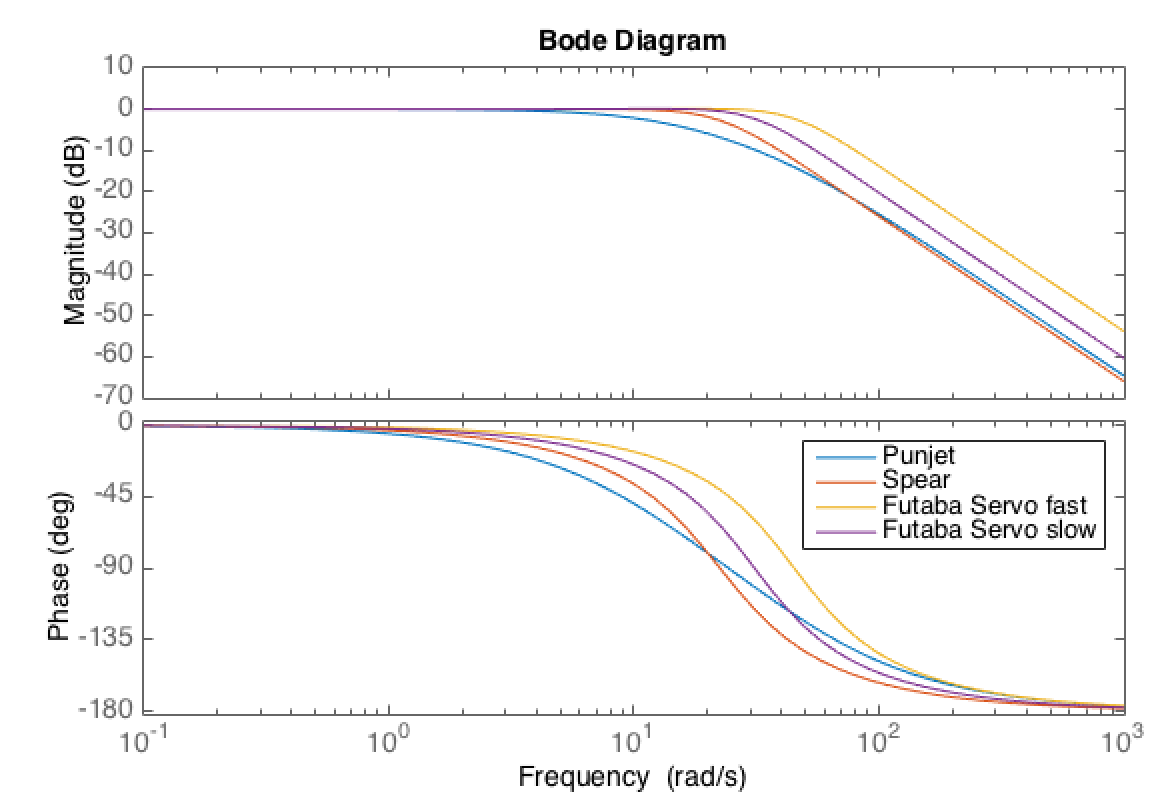
\includegraphics[width=0.85\textwidth]{bode_analysis.png}
  \caption{Aircraft Frequency Analysis }
  \label{fig:bode_analysis}
\end{figure}

These rough approximations were used to then place the cutoff frequencies of the companion model with the expectation that the companion model cannot achieve higher bandwidths than that of the airframe.  Conservatively, the companion model cutoff frequency was typically set 2-5 $rad/s$ lower than the expected max performance of the airframe.  After the other algorithm gains are tuned, and satisfactory performance is achieved, the companion model cutoff frequency can then be increased to achieve higher performance.

\section{Improved Recursive Architecture}

The speed of adaptation and accuracy of the discretized \Lone algorithm is drastically improved with increased loop frequency.  The algorithm was written as one recursive architecture that updates at the Pixhawk's scheduled loop rate.  As previously discussed, the scheduled loop rate ideally should run at lower frequencies to prevent excessive log file size and added strain on the CPU.  However, the \Lone architecture only requires the adaptation loop be run at faster rates.  With this specific performance enhancement in mind, the \ac{APM} architecture could be modified to accept an independent loop specifically for the \Lone adaptation update.  The sensors measurements and \ac{EKF} update can run significantly lower with only increased performance of the algorithm.  The higher adaptation loop would enable higher adaptation gains $(\Gamma)$ and consequently produce faster adaptation of the system.

\section{Integrator Windup Issue}
The \Lone controller architecture exhibits a similar response to integrator wind up in \ac{PID} control when the aircraft is not flying.  If the controller was enabled before takeoff, the control surfaces would move to counteract any slight deviation from input to output attempting to zero the error. Because the aircraft was not flying, the controller would continue to increase the control output until the actuators reached saturation.  The baseline code was configured to ensure that the parameter estimates would not continue to integrate after saturation was reached.  This technique is standard practice when writing control laws that utilize actuators that have saturation limitations.  However, the anti-windup feature that this offers only occurs when the actuators are saturated.  This is inadequate for the takeoff scenario.  The flight surfaces quickly saturate while waiting for takeoff and cause a crash immediately upon takeoff.  It is standard practice to also disable the integrator action of controllers if it is known that the aircraft is not flying using any combination of airspeed, throttle position, \ac{IMU} estimated velocity, or \ac{GPS} ground speed.  In the case of the \Lone algorithm, the integrator utilized in $D(s)$ is essential to the entire architecture and presented challenges in how to use ad-hoc methods to prevent the integrator windup issue even though the 'non-flying' state was calculable onboard the autopilot.  The initial experiments were to see if the adaptation rate was fast enough to un-learn the aircraft's saturated state, but there were no combinations of filter gains which resulted in learning rates adequate to ensure safe takeoffs.  Further research in this area is required to completely replace the \ac{PID} controller with the \Lone.  All takeoffs were conducted either in manual control or with the \ac{PID} controller enabled until safely airborne.

In summary, no one manual has been created for this type of controller's implementation and integration.  The recommendations provided may only apply to this specific implementation of the \Lone adaptive controller, but it offers guidance where none previously was articulated in contemporary literature.
